\documentclass[11pt]{article}

\usepackage{amsmath,amssymb}
\usepackage{a4wide}
\usepackage{graphicx}
\usepackage{tikz}
\usepackage{caption}
\usepackage{subcaption}
\usepackage{gensymb}



\begin{document}
\section{The algorithms}
\label{se:algorithms}
\subsection{Network Algorithm}
\subsubsection{Outline}
The algorithm consists of the following steps:
\begin{enumerate}
  \item Compute the $EMST$ of $P$.
  \item Find points with degree 1 and connect, if possible, to a nearby node.
  \item Find segment that divert from straight roads and remove these segments from the graph.
  \item After removing segments, find better segments to connect the road network.
\end{enumerate}
  
\subsubsection{Description}
Given the set $P$ that contains $n$ points in $\mathbb{R}^2$ first the Eucledian minimum spanning tree $EMST$ is calculated using Prim's algorithm \cite{p-scnsg-57}, in $O(n^2)$ time and $O(n)$ storage. This results in a connected graph $RN(P,S)$, where $s_{a,b}\in S$ represents a road segment between points $a,b \in P$. This gives a good approximation of the road network but some road segments may be missing, see figure \ref{emst}.

\begin{figure}[h]
  \centering
      \graphicspath{ {images/}}
      \includegraphics[width=0.5\linewidth]{NetworkMST}
      \caption{$EMST$ for a given set $p$. The red dashed circles indicate the missing road segments.}
      \label{emst}
  \end{figure}

From $RN$ a new graph is made in which the missing road segments are added in a naive way. For each point $p_1 \in P$ that has degree $1$ the nearest point $p_n \in Adj_{p_1,5}$ is found such that the angle between the segment that contains $p_n$ and point $p_n$ is greater than $90\degree$. This avoids that roads contain sharp angles. A minimum spanning tree has at most $n-1$ points with degree 1 \cite{clrs-ia-09}, this step takes $O(n)$ time in the worst case. 

The next step in the algorithm is to find road segments that diverge from straight roads. $\alpha_{straight}$ is defined as the minimum angle for which two consecutive road segments are considered as a straight road. $\alpha_{min}$ is the minimum angle that a road segment must make with the previous segment for it not to be a bend. For every point $p_2 \in P$ that has degree $2$ there are two points $r_1, q_1 \in P$ which make up the segments $s_{p_2, q_1}$ and $s_{p_2,r_1}$. Segments $s_{q_1, q_2}$ and $s_{r_1,r_2}$ are the segments that are connected to $q_1$ and $r_1$. Let $\theta=\varphi(s_{p_2, q_1},s_{p_2,r_1})$. If $\theta> \alpha_{straight}$ then $\alpha_1=\varphi(s_{p_2, q_1},s_{q_1, q_2})$ and $\alpha_2=\varphi(s_{p_2, r_1},s_{r_1, r_2})$, see figure \ref{networkremove}. If $\alpha_1$ or $\alpha_2$ $<\alpha_{min}$ then $s_{r_1, r_2}$ or $s_{q_1, q_2}$ is removed from $S$. Every point is visited once and finding the segment that include this point takes $O(|S|)$, since $|S|<n$ the upper bound is then $O(n)$. This gives running time of $O(n^2)$ for this step.

\begin{figure}[h]
\centering
  \graphicspath{ {images/}}
  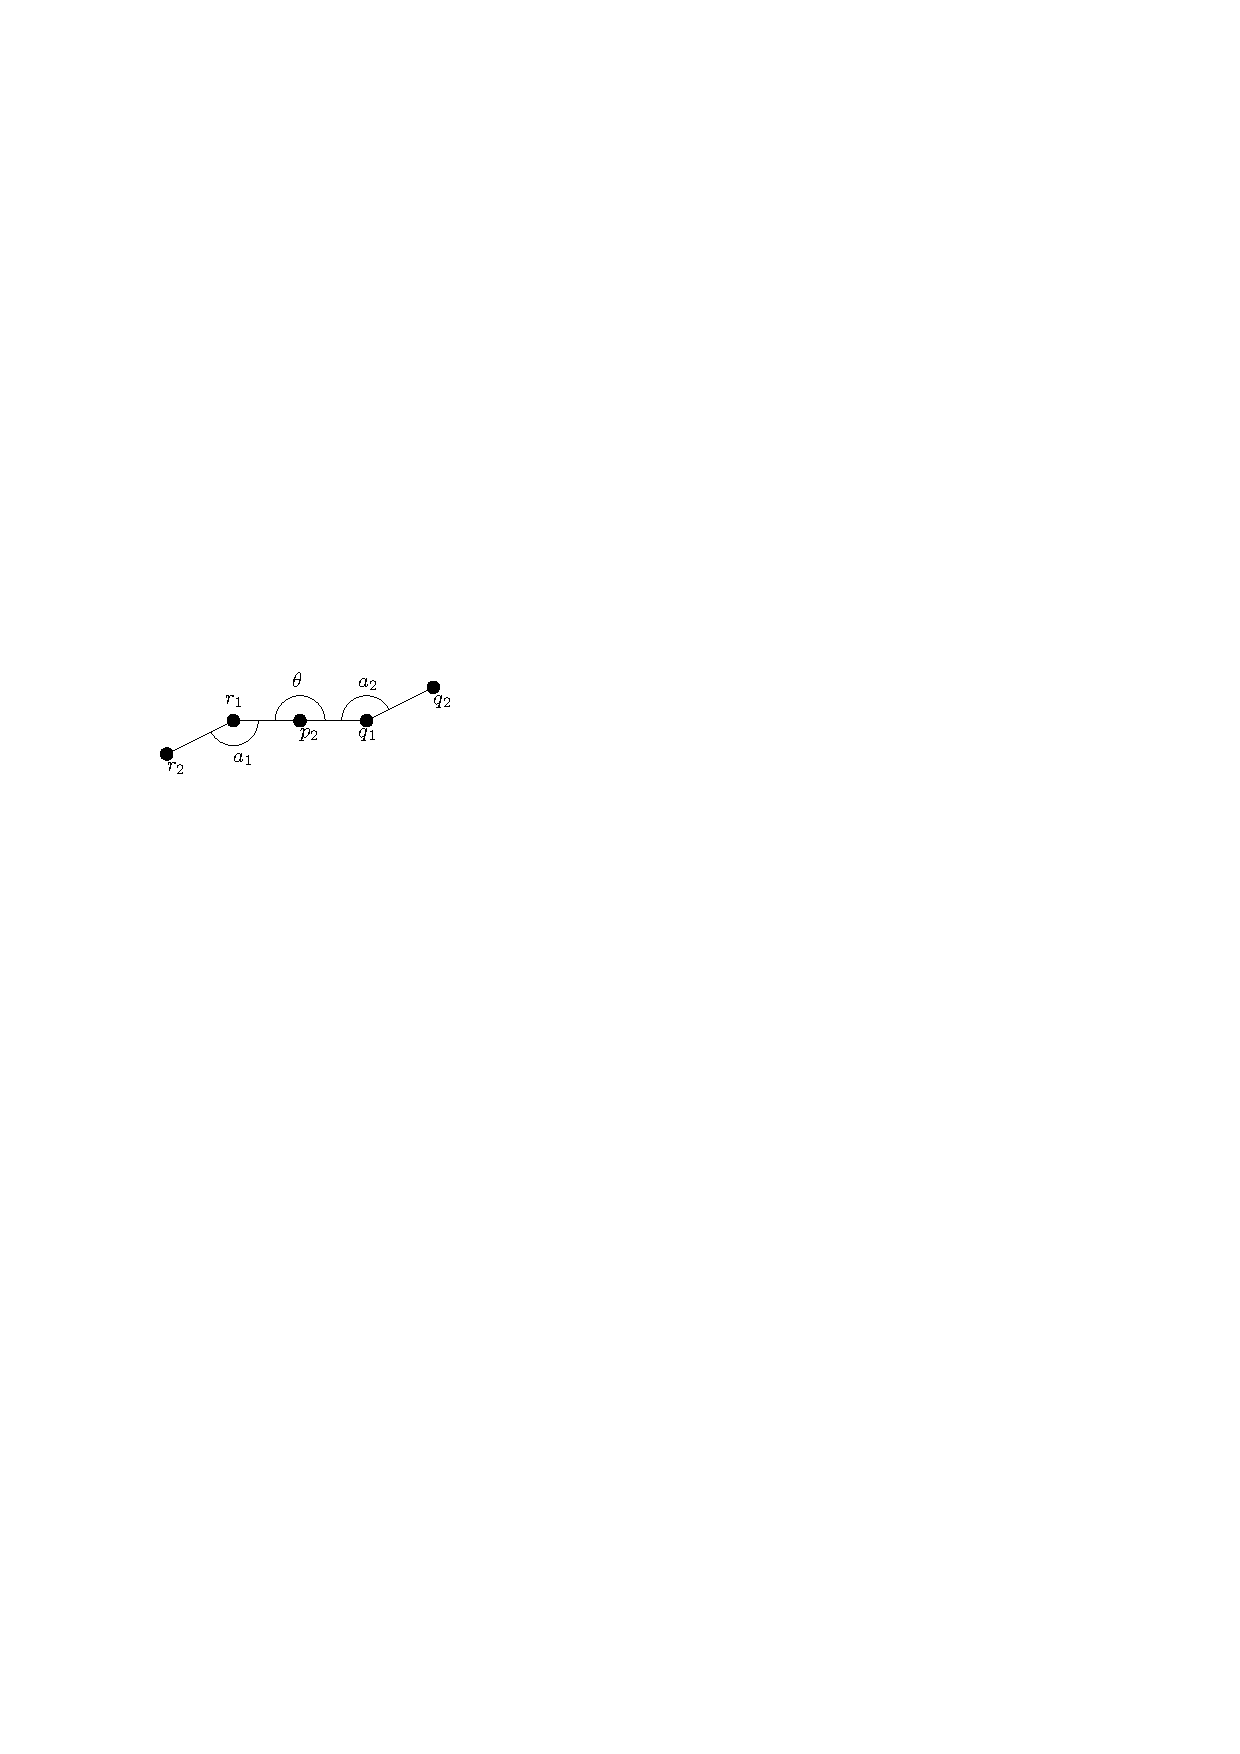
\includegraphics[width=0.5\linewidth]{NetworkRemoveSegmentsDetail}
  \caption{Schematic of $\theta$, $\alpha_1$ and $\alpha_2$}
  \label{networkremove}
\end{figure}
  
$RN$ is now an unconnected graph. For $RN$ to represent the road network it must be connected. Points that are not connected have degree 1. $d_{max}$ is defined as the maximum distance that is allowed between two points for them to form a new segment. For every point $p_3 \in P$ that has degree 1, the 10 most nearest points are found. $q_3 \in P$ is the point such that $s_{q_3, p_3} \in S$. Let $p_{near} \in Adj_{p_3,10}$ be such a point and $\alpha_3=\varphi(s_{q_3, p_3},s_{p_3, p_{near}})$. If $\alpha_3>\alpha_{min}$, $d(p_3,p_{near})<d_{max}$ and $s_{p_3, p_{near}}$ does not intersect any other segment in $S$ then $S=S \cup \{s_{p_3, p_{near}}\}$. In case a intersection does occur at point $u_1 \in U$ with segment $s_{w_1, w_2}\in S$, $P_{add}=P_{add}\cup \{u\}$. Four new segments $s_{w_1, u_1}$, $s_{u_1, w_2}$, $s_{p_3, u_1}$ and $s_{u_1, p_{near}}$ are added to $S$ and $s_{w_1, w_2}$ is removed from $S$, see figure \ref{addintersect}.

\begin{figure}[h]
\centering
      \graphicspath{ {images/}}
      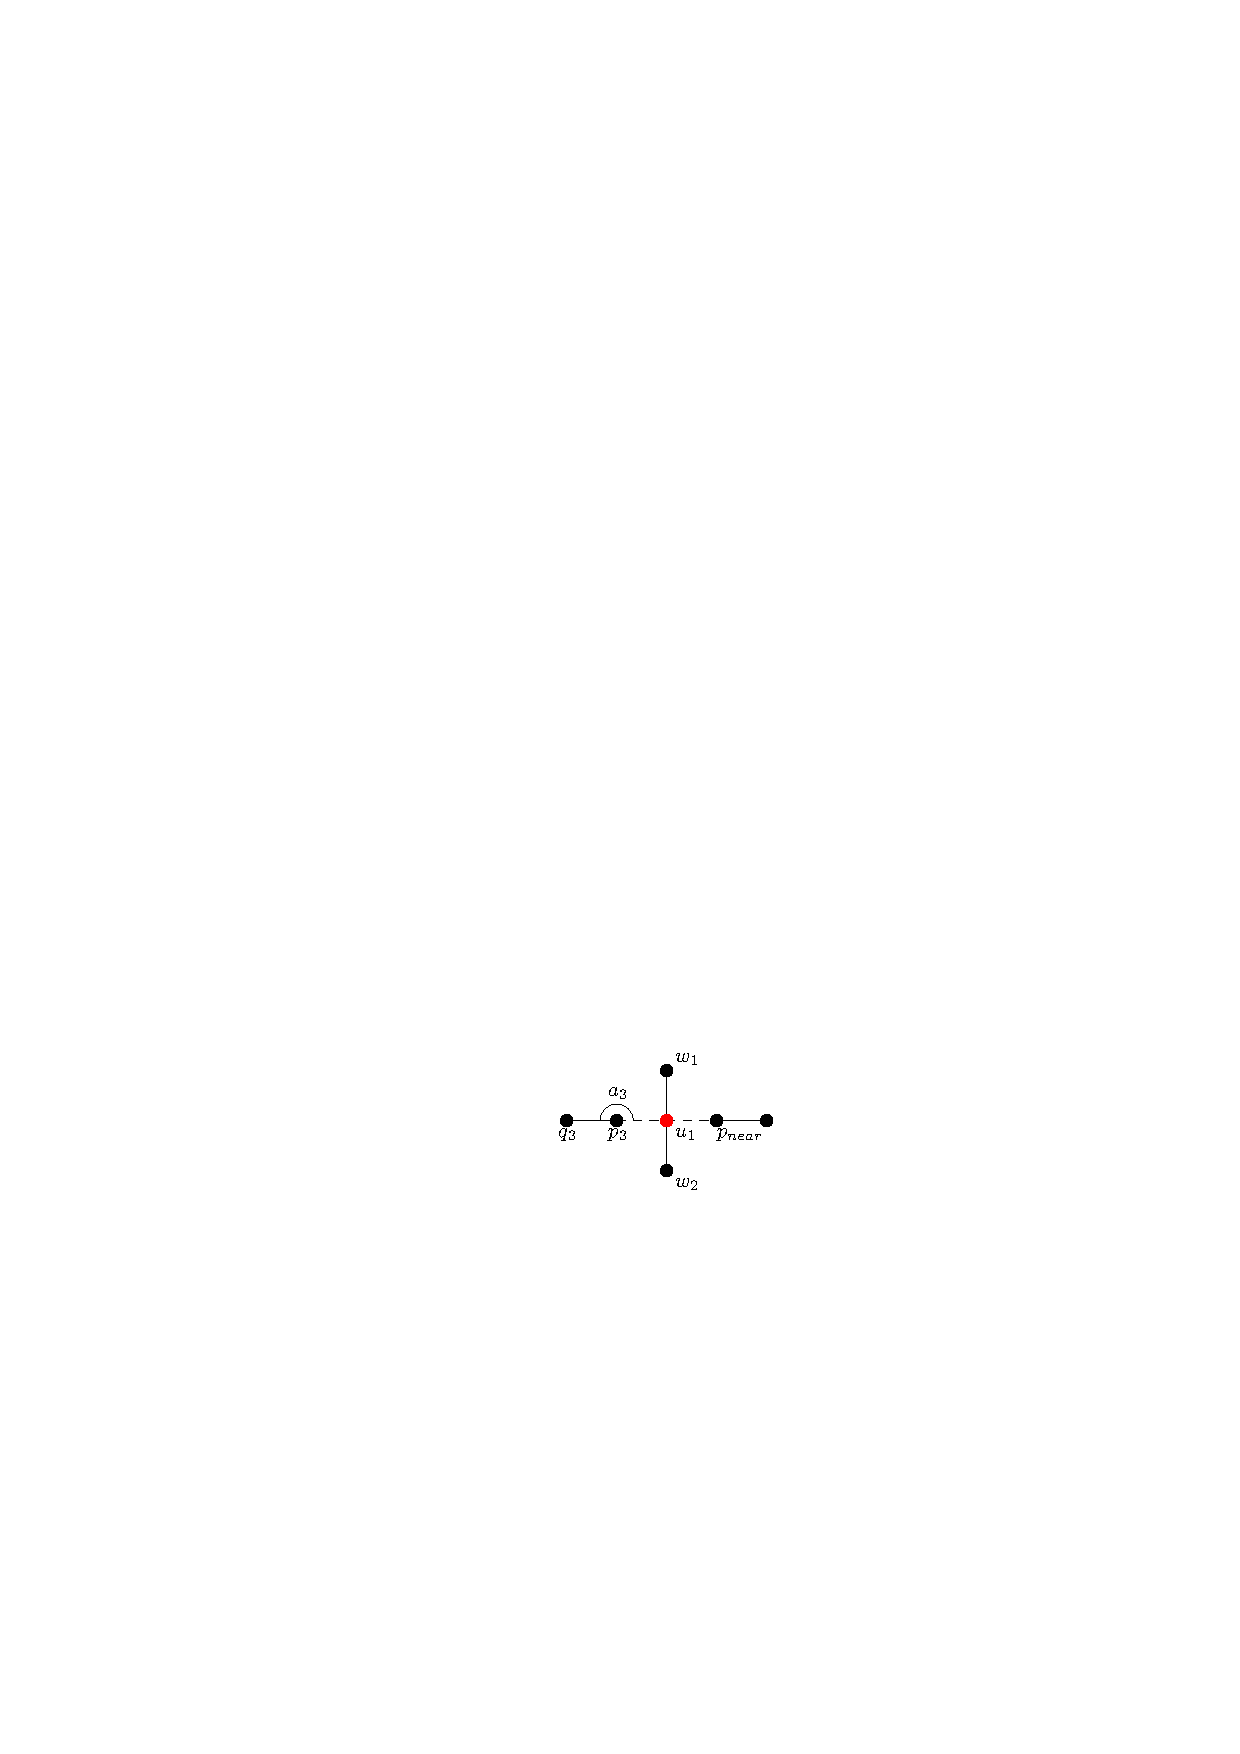
\includegraphics[width=0.5\linewidth]{NetworkAddIntersection}
      \caption{Adding a new segment that intersects the existing segment $s_{w_1,w_2}$}.
      \label{addintersect}
  \end{figure}

When no such point is found in $Adj_{p_3,10}$ the segment $s_{q_3, p_3}$ is extended, in the same direction, with a new segment $s_{p_3,q_4}$ where $q_4 \in U$ and $d(p_3,q_4)=d_{max}$. If $s_{p_3,q_4}$ intersects with another segment $s_{w_3,w_4} \in S$ at $u_2 \in U$ then three new segments $s_{p_3,u_2}$, $s_{w_3,u_2}$ and $s_{u_2,w_4}$ are added to $S$, $s_{w_3,w_4}$ is removed from $S$ and $P_{add}=P_{add}\cup \{u_2\}$. Every point with degree 1 is visited, in the worse case these are all points. For every point at most 10 points are looked up in the adjacency list. Comparisons between the points takes $O(1)$. This gives a running time of $O(n)$.

If we add the running times for each step that gives us: $O(n^2)+O(n)+O(n^2)+O(n)=O(n^2)$. The first step of the algorithm creates a minimum spanning tree that uses $O(n)$ storage. In the second step at most $n-1$ segments are added. The last step only creates a new segment if another segment is removed. The adjacency lists take $O(mn)$ storage, where $m$ is the number of nearby points to store. Since this is a constant the adjacency lists use $O(n)$ storage. Combining these results gives a total storage of $O(n)$.

\subsubsection{Evaluation}
For this experimental evaluation the algorithm was run on several different input sets and with different parameters. The parameter $d_{max}$ is equal to the average length of the segments of the $EMST$ multiplied by a constant. Experimental evaluation showed that this constant should be around $2.5$. The parameter $\alpha_{straight}$ is set to $170\degree$ and $\alpha_{min}$ is set to $165\degree$. In the experimental evaluation below it shown that these values give the best result overall.
\begin{figure}[h]
\centering
  \begin{subfigure}{.4\linewidth}
  \centering
  \graphicspath{ {images/}}
  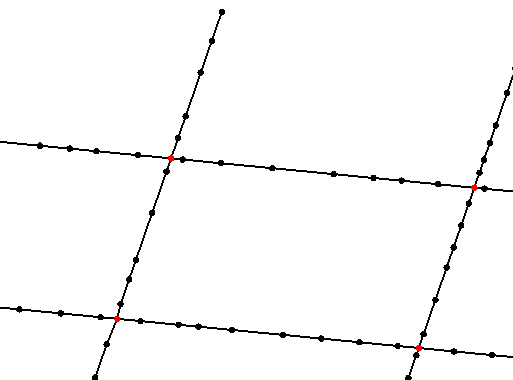
\includegraphics[width=\linewidth]{given167_170}
  \caption{$\alpha_{min}=165$ and $\alpha_{straight}=170$. }
  \label{givena}
  \end{subfigure}
    \begin{subfigure}{0.4\linewidth}
  \centering
  \graphicspath{ {images/}}
  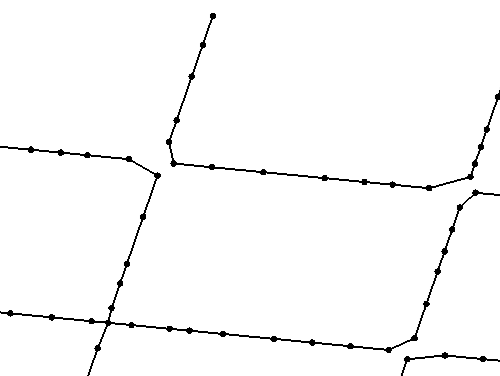
\includegraphics[width=\linewidth]{given90_90}
  \caption{$\alpha_{min}=130$ and $\alpha_{straight}=170$.}
  \label{givenb}
  \end{subfigure}
  \caption{}
  \label{given}
\end{figure}

Figure \ref{given} shows the output of the algorithm of a test case with straight roads and junctions. \ref{givena} shows the output with $\alpha_{min}=165$ and $\alpha_{straight}=170$ and \ref{givenb} shows the output with $\alpha_{min}=90$ and $\alpha_{straight}=170$. A crucial step in the algorithm is to identify straight road segments. A straight road segment consists of three points that make up two consecutive segments of which the middle point has degree 2. For a perfectly straight road the angle between these two segment is $180\degree$. But in our input straight roads could have a slight bend, therefore we set a margin of $10\degree$ by setting $\alpha_{straight}=170$. It is clear that figure \ref{givena} gives a better solution than figure \ref{givenb}. In figure \ref{givenb} any angle greater than $130\degree$ between two consecutive road segment is allowed. In figure \ref{givena} only angles greater than $165\degree$ between two consecutive road segments are allowed. Therefore the segments with a smaller angle, that were not removed in figure \ref{givenb}, are removed and connected to a point that gives an angle smaller than $165\degree$.

\begin{figure}[h]
\centering
  \begin{subfigure}{0.4\linewidth}
  \centering
  \graphicspath{ {images/}}
  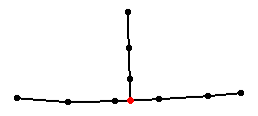
\includegraphics[width=\linewidth]{test1165_170}
  \caption{$\alpha_{min}=165$ and $\alpha_{straight}=170$.}
  \label{tjunctiona}
  \end{subfigure}
    \begin{subfigure}{0.4\linewidth}
  \centering
  \graphicspath{ {images/}}
  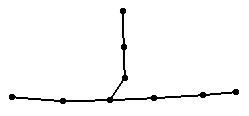
\includegraphics[width=\linewidth]{test1140_170}
  \caption{$\alpha_{min}=160$ and $\alpha_{straight}=170$.}
  \label{tjunctionb}
  \end{subfigure}
  \caption{}
\label{tjunction}
\end{figure}

Figure \ref{tjunction} shows a specific situation of a t-junction. With $\alpha_{min}=160$ the divergent segment in figure \ref{tjunctionb} is not removed. But with $\alpha_{min}=165$ the segment is removed, see figure \ref{tjunctiona} and a segment is added that connects to the new red point. Thus the angle, between the divergent segment and the segment above it, is greater than $160\degree$ and smaller than $165\degree$.  It is arguable that the divergent segment should be removed because a real road could have a slight bend towards a t-junction. By observing several cases $\alpha_{min}=165$ seems close to the optimal setting.

\begin{figure}[h]
\centering
  \begin{subfigure}{0.4\linewidth}
  \centering
  \graphicspath{ {images/}}
  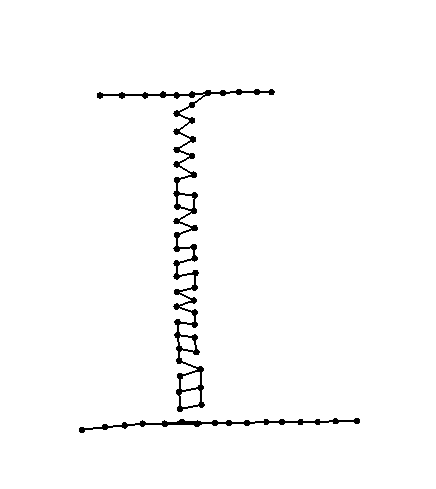
\includegraphics[width=\linewidth]{parallel165_165}
  \caption{$\alpha_{min}=165$ and $\alpha_{straight}=170$.}
  \label{parallel}
  \end{subfigure}
    \begin{subfigure}{0.4\linewidth}
  \centering
  \graphicspath{ {images/}}
  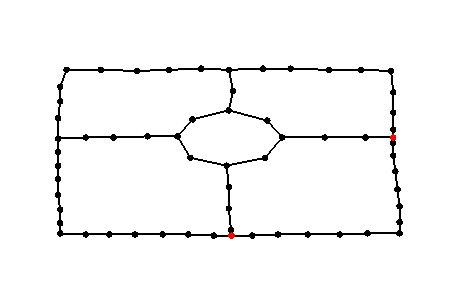
\includegraphics[width=\linewidth]{roundabout167_170}
  \caption{$\alpha_{min}=165$ and $\alpha_{straight}=170$.}
  \label{roundabout}
  \end{subfigure}
  \caption{}
  \label{testcases}
\end{figure}

In figure \ref{testcases} two different cases are shown. In the first case, figure \ref{parallel}, it is clear that the algorithm doesn't give an optimal solution. The algorithm's initial step creates a $EMST$, thus connecting the points with minimum total distance. This doesn't work well for parallel roads if the distance between the points that belong the same road is greater than the distance between points from both roads. The $EMST$ then connects the points that are closest to each other and thus connects points that should be in different roads. The next step of the algorithm looks for straight road segments and tries to improve the road network from there. However, as figure \ref{parallel} shows, the two parallel roads do not contain a straight road consisting of two straight segments of which the middle point has degree 2. Therefore the algorithm is not able to improve on this solution.

Figure \ref{roundabout} shows a test case with a roundabout and several t-junctions. The algorithm seems the give the optimal solution for this particular input. The roundabout is created by the first two steps of the algorithm. First the $EMST$ is created which nearly completes the roundabout and then point with degree 1 are connected to a nearby point, which works very well in this case. Also the t-junctions are connected in the right way with the given parameters.

\begin{figure}[h]
  \centering
  \graphicspath{ {images/}}
  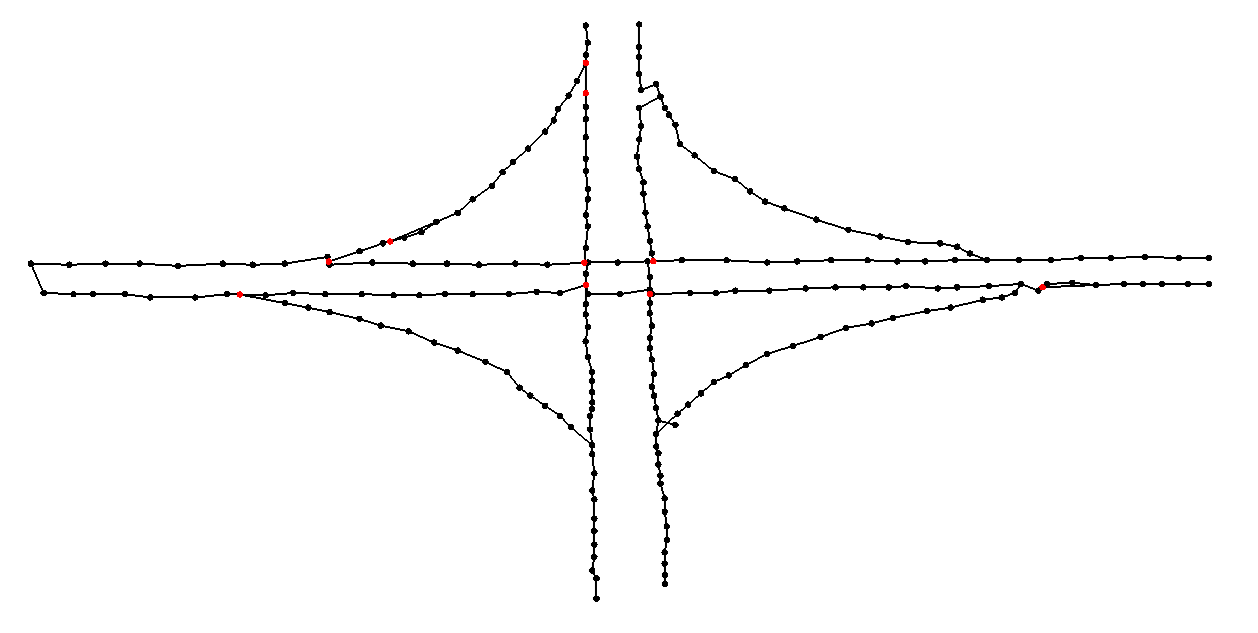
\includegraphics[width=\linewidth, height=150pt]{knooppunt167_170}
  \caption{$\alpha_{min}=165$ and $\alpha_{straight}=170$.}
  \label{knooppunt}
\end{figure}

Figure \ref{knooppunt} shows an input case with parallel roads for which the algorithm gives a fairly good solution. Because there is some space between the two parallel roads the $EMST$ doesn't connect two points that don't belong to the same road.

\subsection{conclusion}
The experimental evaluation showed that the algorithm doesn't always give the optimal solution, but in most cases it comes close and sometimes it does give the optimal solution. The algorithm works very well for junctions and t-junctions, if the parameters are set correctly, which can be seen clearly in figure \ref{givena} and figure \ref{tjunctiona}. For parallel roads it doesn't always give an optimal solution, especially when the two roads are close to each other. This can be seen in figure \ref{parallel}. In cases where there is more distance between two parallel roads the algorithm works fairly well, as can be seen in figure \ref{knooppunt}. In future work the output for cases with parallel roads could be improved.

\bibliographystyle{plain}

\begin{thebibliography}{}

\bibitem{p-scnsg-57}
R. C. Prim.
Shortest connection networks and some generalizations.
In \emph{Bell System Technical Journal)}, 36: (1957), pp. 1389–1401

\bibitem{clrs-ia-09}
T.H. Cormen, C.E. Leiserson, R.L. Rivest, C. Stein.
\emph{Introduction to Algorithms} (3th edition).
The MIT Press, 2009.

\bibitem{cghs-rnrop-20}
D. Chen, L.J. Guibas, J. Hershberger, J. Sun.
Road Network Reconstruction for Organizing Paths.
In \emph{Proceedings  of  21st  ACM-SIAM  Symposium  on  Discrete  Algorithms}, 10: 1309-1320, 2010.
\end{thebibliography}
\end{document}
